\documentclass[tikz,border=4pt]{standalone}
% Estilos compartilhados pelos diagramas dos estágios e módulos do Core.
\usetikzlibrary{arrows.meta, positioning, calc, shapes.geometric, fit}

\tikzset{
  >={Stealth[length=2.2mm]},
  bloco/.style={draw, rounded corners=2pt, minimum width=24mm, minimum height=9mm,
                align=center, font=\small, fill=blue!6},
  regpipe/.style={draw, minimum width=9mm, minimum height=48mm, align=center,
                  font=\small, fill=gray!25},
  mux/.style={draw, trapezium, trapezium angle=70, shape border rotate=90,
              minimum height=11mm, minimum width=7mm, inner sep=1pt, align=center,
              font=\scriptsize, fill=orange!15},
  ctrl/.style={draw, rounded corners=2pt, minimum width=24mm, minimum height=9mm,
               align=center, font=\small, fill=green!10},
  opcional/.style={bloco, dashed, fill=yellow!12},
  externo/.style={draw, rounded corners=2pt, minimum width=24mm, minimum height=9mm,
                  align=center, font=\small, fill=red!8},
  dado/.style={->, thick},
  sinal/.style={->, dashed},
  rotulo/.style={font=\scriptsize, midway, above, inner sep=1pt},
  titulo/.style={font=\bfseries\normalsize}
}

\begin{document}
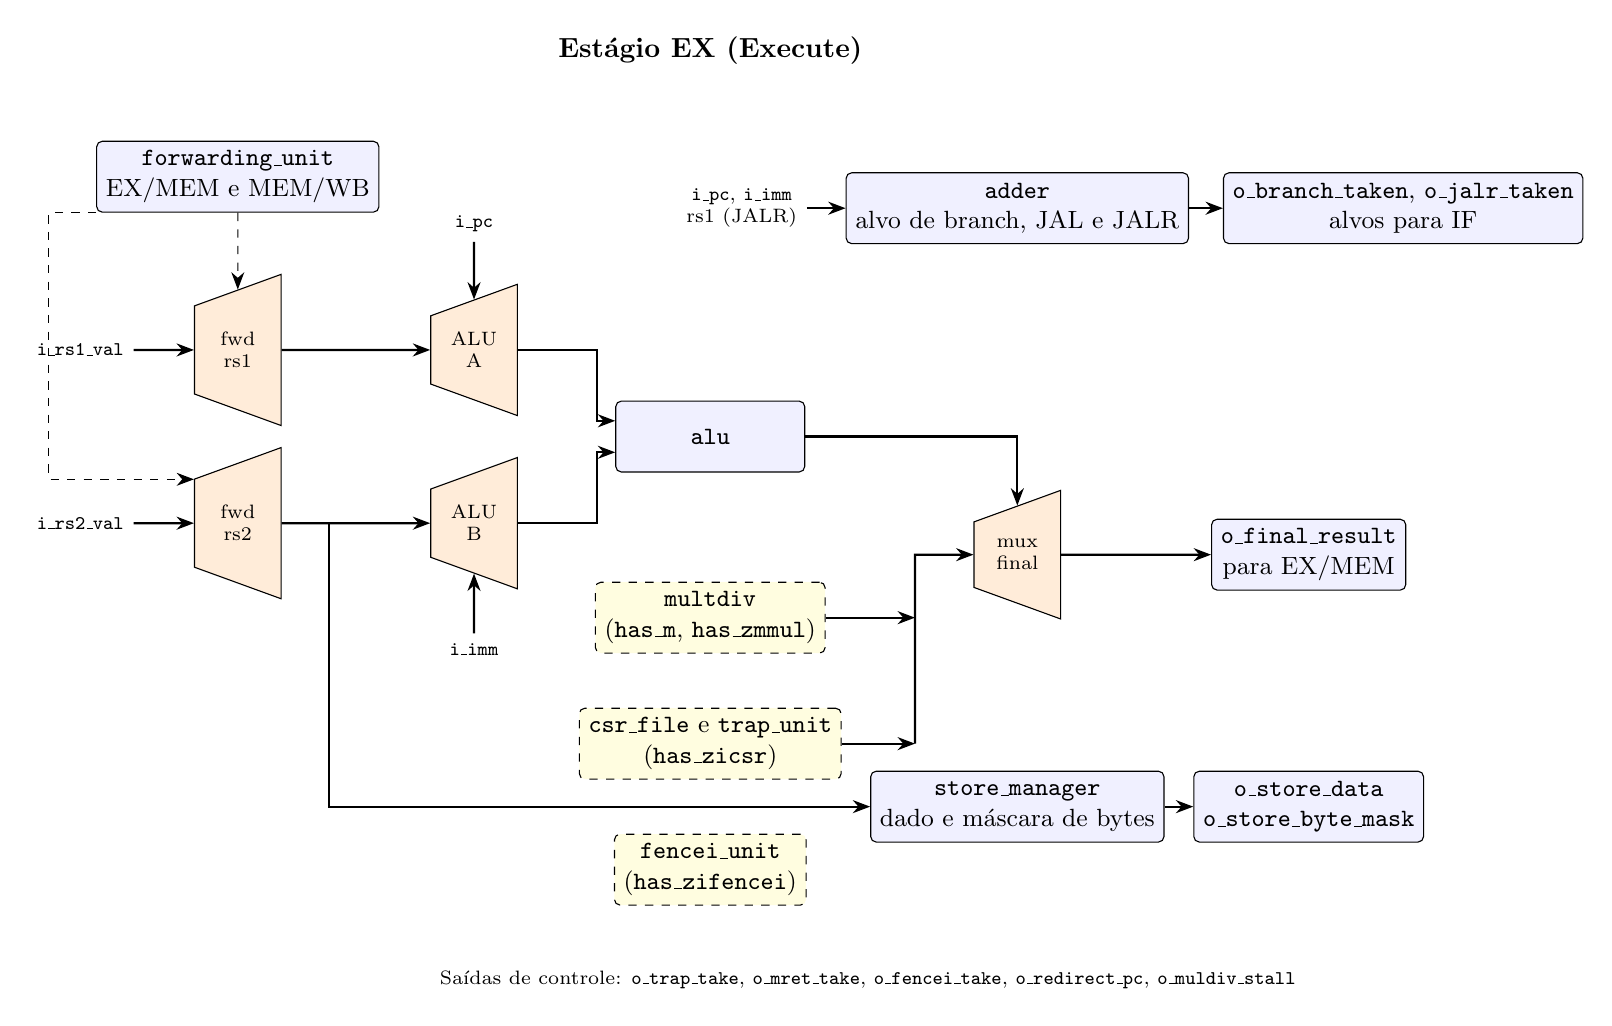
\begin{tikzpicture}
  \node[titulo] at (8,7.4) {Estágio EX (Execute)};
  \node[bloco] (fwd) at (2,5.8) {\texttt{forwarding\_unit}\\EX/MEM e MEM/WB};
  \node[mux] (f1) at (2,3.6) {fwd\\rs1};
  \node[mux] (f2) at (2,1.4) {fwd\\rs2};
  \node[mux] (a) at (5,3.6) {ALU\\A};
  \node[mux] (b) at (5,1.4) {ALU\\B};
  \node[bloco] (alu) at (8,2.5) {\texttt{alu}};
  \node[opcional] (md) at (8,0.2) {\texttt{multdiv}\\(\texttt{has\_m}, \texttt{has\_zmmul})};
  \node[opcional] (csr) at (8,-1.4) {\texttt{csr\_file} e \texttt{trap\_unit}\\(\texttt{has\_zicsr})};
  \node[opcional] (fi) at (8,-3.0) {\texttt{fencei\_unit}\\(\texttt{has\_zifencei})};
  \node[mux] (fin) at (11.9,1.0) {mux\\final};
  \node[bloco] (bt) at (11.9,5.4) {\texttt{adder}\\alvo de branch, JAL e JALR};
  \node[bloco] (sm) at (11.9,-2.2) {\texttt{store\_manager}\\dado e máscara de bytes};
  \node[bloco] (out) at (15.6,1.0) {\texttt{o\_final\_result}\\para EX/MEM};
  \node[bloco] (br) at (16.8,5.4) {\texttt{o\_branch\_taken}, \texttt{o\_jalr\_taken}\\alvos para IF};
  \node[bloco] (st) at (15.6,-2.2) {\texttt{o\_store\_data}\\\texttt{o\_store\_byte\_mask}};
  \node[font=\scriptsize, align=right] (rs1) at (0,3.6) {\texttt{i\_rs1\_val}};
  \node[font=\scriptsize, align=right] (rs2) at (0,1.4) {\texttt{i\_rs2\_val}};
  \node[font=\scriptsize] (pc) at (5,5.2) {\texttt{i\_pc}};
  \node[font=\scriptsize] (imm) at (5,-0.2) {\texttt{i\_imm}};
  \node[font=\scriptsize, align=center] (btin) at (8.4,5.4) {\texttt{i\_pc}, \texttt{i\_imm}\\rs1 (JALR)};

  \draw[dado] (rs1) -- (f1);
  \draw[dado] (rs2) -- (f2);
  \draw[sinal] (fwd) -- (f1);
  \draw[sinal] (fwd.south west) -- ++(-0.6,0) |- (f2.north west);
  \draw[dado] (f1) -- (a);
  \draw[dado] (f2) -- (b);
  \draw[dado] (pc) -- (a.north);
  \draw[dado] (imm) -- (b.south);
  \draw[dado] (a.east) -- ++(1.0,0) |- ([yshift=2mm]alu.west);
  \draw[dado] (b.east) -- ++(1.0,0) |- ([yshift=-2mm]alu.west);
  \draw[dado] (alu.east) -| (fin.north);
  \draw[dado] (md.east) -- (10.6,0.2);
  \draw[dado] (csr.east) -- (10.6,-1.4);
  \draw[dado] (10.6,-1.4) -- (10.6,1.0) -- (fin.west);
  \draw[dado] (fin) -- (out);
  \draw[dado] (btin) -- (bt);
  \draw[dado] (bt) -- (br);
  \draw[dado] (f2.east) -- ++(0.6,0) |- (sm.west);
  \draw[dado] (sm) -- (st);
  \node[font=\scriptsize, align=left] at (10,-4.4) {Saídas de controle: \texttt{o\_trap\_take}, \texttt{o\_mret\_take}, \texttt{o\_fencei\_take}, \texttt{o\_redirect\_pc}, \texttt{o\_muldiv\_stall}};
\end{tikzpicture}
\end{document}
